\documentclass{article}
\usepackage[utf8]{inputenc}
\usepackage{graphicx}
\usepackage{float}
\usepackage{biblatex}
\usepackage{Qcircuit}
\usepackage{amsmath}
\usepackage{xy}

\title{Proving that three qubit error correction of a single qubit has occurred in a simulated quantum system}
\author{physicsnerd\footnote{no academic or industrial affiliation}}
\date{February 26, 2017}

\addbibresource{sample.bib}
\graphicspath{{images/}}

\begin{document}

\maketitle

\begin{abstract}
    In this paper it is shown that the bit-flip error correction code corrects an artificially introduced error of a single qubit in a quantum system simulated using Quirk. To prove that error correction has been done it is shown that in the simulation the qubit returns the same state as the one it was initialized in, and second that the mathematical representation of the qubit's states and the gates applied to them corresponds with the simulation.
\end{abstract}

\section{Introduction}
Quantum computing uses the principles of quantum mechanics to solve problems that cannot be solved classically.\cite{chuang}
It is only useful for certain, specialized problems, such as (famously) finding the prime factorization of numbers swiftly.\cite{shor} 
Quantum computing is fundamentally the performance of various operations on qubits, the quantum equivalent of a bit. 
These qubits are very small, so that the principles of quantum mechanics can be employed. 
This brings with it its own problems. Any amount of noise within the system could interfere with the qubits and cause an erroneous result to the problem.
Further, qubits have the problem of decoherence - they only stay stable for a short length of time.\cite{decoherence}

As the problems quantum computers are attempting to solve and the algorithms they are attempting to run get more and more complex, take longer, and require more qubits, the problem of noise and decoherence only increases.
Error correction is used to account for noise and decoherence and correct the errors that arise mid-calculation.\cite{decoherence}
There are various error correcting codes that "shuffle over" the error from the qubit used in the calculation to other qubits used specifically for that purpose. 
(The error cannot be totally removed as that would decrease entropy.)

\section{Theory}
\subsection{Quantum Channels}
Quantum channels are communications channels that can transfer classical and quantum information.\cite{channel} Due to noise and decoherence, there is a small probability of qubits being flipped as they pass through the channel. The quantum channel is simulated by artificially flipping a qubit via a NOT (or Pauli-X) gate. 
\subsection{Bit-Flip Code}
The bit-flip code is a three qubit error correction code. One qubit goes in in a state $|\psi\rangle$. 
The qubit is then entangled with two qubits, both in the state $|0\rangle$, through the use of two CNOT (controlled-NOT) gates. 
The qubits then go through a quantum channel $E_{\mathrm{bit}}$, which has a small probability of changing one of the qubits' state.\cite{qcqi}
Here it is assumed that at most one bit flip can occur. 

Syndrome diagnosis is then used to determine which, if any, of the qubits got flipped without disturbing the quantum states. To do this, two CNOT gates are used as projection operators, which compare each of the qubits, see which (if any) are different, and allow the user to determine which qubit is different. The Toffoli gate then flips the incorrect qubit (if there is one) back to its proper state. (See Figure 1 for a diagram.)\cite{qcqi}

\begin{figure}[H]
    \begin{align*}
 \Qcircuit @C=1em @R=.7em {
  \lstick{\ket{\psi}} & \ctrl{1} & \ctrl{2} & \multigate{2}{E_{\text{bit}}} & \ctrl{1} & \ctrl{2} & \targ     & \rstick{\ket{\psi}} \qw\\
  \lstick{\ket{0}}    & \targ    & \qw      & \ghost{E_{\text{bit}}}        & \targ    & \qw      & \ctrl{-1} & \qw \\
  \lstick{\ket{0}}    & \qw      & \targ    & \ghost{E_{\text{bit}}}        & \qw      & \targ    & \ctrl{-2} & \qw
 }
\end{align*}
\caption{The circuit for the bit-flip code.\cite{wiki}}
\end{figure}

\section{Simulation}
For the simulation, the simulator Quirk was used.\cite{quirk}
\subsection{Setup}
In the simulation, all qubits were initialized in the $|0\rangle$ state. The first qubit (which will be referred to as $Q_0$) then has a NOT gate applied to it, representing previous calculations that may have involved $Q_0$ and also providing a way to test the bit-flip code with multiple inputs. The bit flip code was applied as described in Section 2.3, with a NOT gate simulating the quantum channel ($E_{\mathrm{bit}}$). At the very end, the measurement gate was used. (See Figure 2.)

\begin{figure}[H]
    \centering
    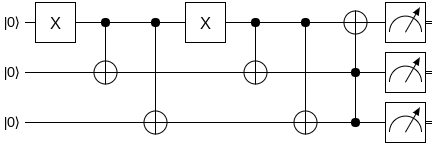
\includegraphics[scale=0.6]{bitflipsimulation.png}
    \caption{The simulation setup.}
    \label{fig:bitflipsimulation}
\end{figure}

Two other simulations were also done, with the same method, with the exception of $Q_0$ having no gate applied to it (see Figure 3) or the Hadamard gate applied to it (see Figure 4).

\begin{figure}[H]
    \centering
    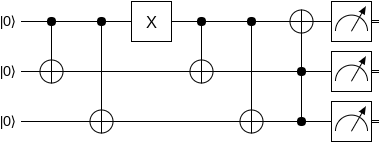
\includegraphics[scale=0.6]{bitflipsimulation2.png}
    \caption{The simulation setup with no gate applied to $Q_0$ in the beginning.}
    \label{fig:bitflipsimulation2}
\end{figure}

\begin{figure}[H]
    \centering
    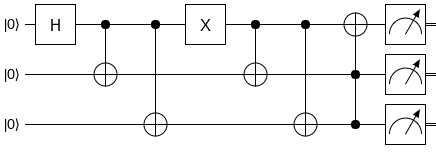
\includegraphics[scale=0.6]{bitflipsimulation3.png}
    \caption{The simulation setup with the Hadamard gate applied to $Q_0$ in the beginning.}
    \label{fig:bitflipsimulation3}
\end{figure}

\subsection{Results}
The results showed that the bit-flip code properly corrected errors introduced into the state of the qubits. $Q_0$, no matter the first gate applied to it, always returned the same value. For the results of the first simulation, where the NOT gate was the first gate applied, see Figure 5. For the results of the second simulation, where no gate was applied before the bit-flip code, see Figure 6. For the results of the third simulation, where the Hadamard gate was the first gate applied, see Figure 7.

\begin{figure}[H]
    \centering
    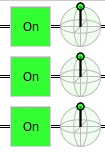
\includegraphics[scale=0.6]{results1.png}
    \caption{The simulation results with the NOT gate applied to $Q_0$ in the beginning.}
    \label{fig:bitflipresults1}
\end{figure}

\begin{figure}[H]
    \centering
    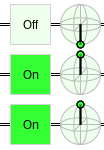
\includegraphics[scale=0.6]{results2.png}
    \caption{The simulation results with no gate applied to $Q_0$ before the bit-flip code.}
    \label{fig:bitflipresults2}
\end{figure}

\begin{figure}[H]
    \centering
    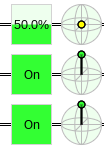
\includegraphics[scale=0.6]{results3.png}
    \caption{The simulation results with the Hadamard gate applied to $Q_0$ in the beginning.}
    \label{fig:bitflipresults3}
\end{figure}

\section{Mathematical Description}
\subsection{Notation}
When notation such as $|110\rangle$ is used, the qubits' states should be read from right to left; i.e., the first qubit is in the zero state, the second in the one state, and the third in the one state. 
When notation such as $\mathrm{NOT}_1$ is used, the subscript lists the qubits to which the gate is applied, i.e., the NOT gate is applied to the first qubit. 
When notation such as $\mathrm{CNOT}_{\mathrm{1,2}}$ is used, control qubits are always listed first; i.e., the first qubit is the control qubit, and the second is the target qubit. 
When notation such as $\mathrm{NOT}_1\to|001\rangle$ is used, the phrase describes what state is produced by gates being applied; i.e., the NOT gate is applied to the first qubit and the state $|001\rangle$ results.

\subsection{Mathematical Examination}
Note that the mathematics of simulation three are analogous to the mathematics of simulations one and two.
\subsubsection{Simulation One}
The qubits are each initialized in the zero state, producing the state $|000\rangle$. In simulation one, the operation $\mathrm{NOT}_1$ is performed, resulting in the state $|001\rangle$. Continuing, the qubits are entangled via $\mathrm{CNOT}_{1,2}\to|011\rangle$ and $\mathrm{CNOT}_{1,3}\to|111\rangle$. The channel is simulated via $\mathrm{NOT}_1\to|110\rangle$. The projection operators are simulated via $\mathrm{CNOT}_{1,2}\to|110\rangle$ and $\mathrm{CNOT}_{1,3}\to|110\rangle$. Finally, the qubit is corrected via $\mathrm{Toffoli}_{2,3,1}\to|111\rangle$.

\subsubsection{Simulation Two}
The qubits are each initialized in the zero state, producing the state $|000\rangle$. In simulation one, the qubits are entangled via $\mathrm{CNOT}_{1,2}\to|000\rangle$ and $\mathrm{CNOT}_{1,3}\to|000\rangle$. The channel is simulated via $\mathrm{NOT}_1\to|001\rangle$. The projection operators are simulated via $\mathrm{CNOT}_{1,2}\to|011\rangle$ and $\mathrm{CNOT}_{1,3}\to|111\rangle$. Finally, the qubit is corrected via $\mathrm{Toffoli}_{2,3,1}\to|110\rangle$.

\subsubsection{Simulation Three}
The qubits are each initialized in the zero state, producing the state $|000\rangle$. In simulation three, the operation $\mathrm{Hadamard}_1$ is performed, resulting in the state $|001\rangle$. Continuing, the qubits are entangled via $\mathrm{CNOT}_{1,2}\to|011\rangle$ and $\mathrm{CNOT}_{1,3}\to|111\rangle$. The channel is simulated via $\mathrm{NOT}_1\to|110\rangle$. The projection operators are simulated via $\mathrm{CNOT}_{1,2}\to|110\rangle$ and $\mathrm{CNOT}_{1,3}\to|110\rangle$. Finally, the qubit is corrected via $\mathrm{Toffoli}_{2,3,1}\to|111\rangle$.

\section{Conclusion}
A working three-qubit error correction code allows for a simple way to correct the errors that arise in more complex calculations. As almost all algorithms require enough qubits that error correction is necessary, it is key that there are codes in the field that require a minimal number of extra qubits and work well. The three qubit code fulfills this requirement. Further research that would improve the bit-flip code tremendously would entail examining the possibility of creating a three qubit code that can account for errors in multiple qubits as they pass through the quantum channel. Examination of the three qubit phase flip code, which can account for errors other than bit flips\cite{qcqi}, is also important. Finally, reducing the number of qubits necessary for the Shor code (a combination of the bit flip and phase flip codes) to work is an important field of study.

\printbibliography

\end{document}
